\chapter{A Realistic 3D Tree Model Based on L-Systems}
\label{chap:treeLsystem}

\noindent
Jie Long and Michael Jones. \emph{A Realistic 3D Tree Model based on L-Systems. Report for UNEP Eco-Peace Leadership Center (EPLC)}, 2008.

\begin{abstract}
Constructing a 3D tree model manually is time consuming due to the natural complexity of tree shapes. We introduce a new morphology-based method using L-systems for realistic 3D tree modeling. Using L-systems for describing tree branches as particles, this method (1) introduces a hemisphere to generate particles, (2) uses a growth level to simulate different ages of branches, and (3) applies a dynamic bounding box to detect local growth area in a tree. This new method enhances the management of tree shapes by easing the control over distributions of branches and leaves. To further validate the method, we demonstrate that the method can simulate photorealism and growth around physical barriers. We evaluate this model by particle flow and by complexity, showing performance competitive with existing methods.
\end{abstract}

\section{Introduction}

The natural complexity of trees has been challenging computer graphics for decades. Many applications---film, 3D video games, city planning, and forestry---require clear, detailed 3D tree models. Although methods exist for creating photorealistic tree models, these methods are still cumbersome. Efficient methods for constructing 3D tree models are needed to deal with the intractable computation of the detailed geometry. Since trees have many properties due to the growth environment and kinds, models with global controls over shapes are also important. 

In recent years, techniques on image-based reconstruction and L-systems have been widely used in 3D tree modeling research. Both methods have advantages and shortcomings. Image-based reconstruction generates natural-looking 3D trees through image processing, but models are limited to trees in the image and most need time-consuming manual modifications. Although L-systems are efficient and easily implement in 2D or 3D tree models, using L-systems representation alone makes it difficult to control small components in a tree (e.g., a certain twig). 

In this paper, we introduce a new method for 3D tree modeling based on L-systems. This new method presents a 3D tree model with three innovations: a hemisphere, level controls, and a dynamic bounding box. First we build a branch library using L-systems. A branch unit, which is also a unit of L-systems and works as a particle, has several twigs. A hemisphere on the top of a tree model controls the distribution of branches and leaves. The growth levels simulate different ages of branches and leaves. A dynamic bounding box constrains the local growth area in a tree by avoiding outer forces. In the implementation, particles are generated on the hemisphere surface and begin to move in the hemisphere with different starting angles. A ray defined by the position and angle of a particle is attracted to the nearest branch in the existing tree. After a new branch attaches to the existing tree, we enlarge the bounding box to the new tree shape. This bounding box grows with the tree volume and can detect collisions with other objects or growth obstacles. In each growth interval, a certain number of branches are generated and distributed. In addition, leaves have initial parameters for shapes, sizes and colors. We also distribute leaves from the hemisphere surface. In each growth stage, leaves have different sizes and colors, but the same shape. 

There are four steps in this 3D tree modeling. First, L-systems generate different branch patterns. Second, a hemisphere designates probability distributions for generating particles. Third, a branch from the branch library is randomly selected, a particle is generated on the designated area, the ray to the tree model is computed, and the nearest growth point is found.  Finally, after constructing branches for the whole tree, leaves with different sizes and colors are added to this model. 

Using this new method, a 3D tree model is more efficient and controllable. We take advantage of L-systems to describe branches for efficiency while overcoming the control scale problem. L-systems and image-based methods control the whole tree at one time. They generate tree models as a whole. However, our method manages small components of a branch, but not the smallest components of twigs. The second advantage of this new method is the ease of control over tree shape. The hemisphere controls distribution probabilities to shape a tree. The bounding box flexibly constrains a proper growth area to detect outer barriers like rocks and buildings. The parameters of a desired shape are far less than existing methods. In addition, our method can distribute leaves with the same shapes but with flexible sizes and colors due to the growth level of branches. Current methods including L-systems and image-based approaches can't manage the age-based distributions of leaves. Also, we carried out a set of experiments to validate this new method: photokinesis simulation and growth around physical barriers. 

\section{Related Work} 

Two main research directions in tree modeling are biology-based and morphology-based. Models that mimic biological data are based primarily on patterns of tree growth. Some tree modeling software, such as AMAP, COSSYM, and SVS, simulate tree growth based directly on biological data.  Morphology-based methods focus on reconstructing tree shapes from photographs or remote sensing (RS) images. Both biology-based and morphology-based methods have applications in different areas. Forestry research uses biology-based models, and 3D games and movies use morphology-based models.  Our system is mainly morphology-based while also considering some biology characteristics of natural trees. In this section, we discuss two primary morphology-based tree modeling methods: L-systems and image-based models.

\subsection{L-systems}

An L-system is a formal grammar that describes the recursive growth of a tree.  The rules of the grammar must be written by the user. Since the rules are applied locally, small changes in the rules may cause large changes in the overall tree shape. Such behavior makes modeling quite difficult. Various extensions of L-systems have been proposed, including parametric \cite{Prusinkiewicz:sv90}, open \cite{Mech:SIGGRAPH96}, and differential L-systems \cite{prusinkiewicz:siggraph93}. These extensions are able to create a variety of effects, but also require additional parameters from the user. Prusinkiewicz et al. \cite{Prusinkiewicz:2001} present a modeling interface for L-systems to enhance the modeling ease, but a large set of parameters still has to be defined by the user.

L-systems have both advantages and shortcomings. L-systems generate 2D and 3D tree models efficiently. This method is easy to implement. However, L-systems generate tree models at one time after defining an algorithm. Further modification of models is difficult. L-systems go too far in simplifying tree models, so the results are not realistic. 

\subsection{Image Reconstructions}

Reconstruction of tree shapes from photographs is an active area of research in 3D tree modeling. 3D tree models from this method look natural because they are based on the morphology of actual trees. People can use 2D source images, which are easily collected using consumer digital cameras, to generate 3D tree models for almost any interesting trees. 

Shlyakhter et al. \cite{shlyakhter:ieeecga01} direct the growth of L-systems using photographs. The registered input images reconstruct a visual hull. The medial axis diagram of the hull constructs the tree skeleton. L-systems describe smaller branches and leaves. 

Reche Martinez et al. \cite{RecheMartinez2004} describe a very precise, though complex, image-based approach. In this case a set of carefully registered photographs determines the volumetric shape of a given tree. The volume is divided into cells; for each cell a set of textures compute a valid visual representation. The complete set of textures represents the tree quite faithfully. 

Neubert et al. \cite{neubert:acmtg07} present a method to produce 3D tree models from 2D photographs using particle flows. Using image information, the author estimates an approximate voxel-based tree volume. Performing a 3D flow simulation, particles form the twigs and branches. The botanical rules for branch thicknesses and branching angles produce the geometry of the tree skeleton. 

Tan et al. \cite{Tan:2007:ITM} propose an approach for generating 3D tree models from images. This method requires little user intervention. This research populates the tree with leaf replicas from segmented source images to reconstruct the overall tree shape. In addition, shape patterns of visible branches can predict those of obscured branches.

\subsection{Other Methods}

There are some other famous approaches for tree modeling.  Aono et al. \cite{Aono:1984} presented the A-system. Oppenheimer \cite{Oppenheimer1986} proposed the animation based on a fractal method. Reeves \cite{ReevesB85} introduced a modeling method based on particle flow. Reffye et al. \cite{deReffye1988,YAN03} presented a model based on botanical structures. Weber et al. \cite{Weber1998} presented a method on generating trees in several steps. Kurth's team \cite{kurth:sf97} developed LIGNUM \cite{Perttunen98} for 3D tree modeling. 

\section{Tree Modeling Using L-systems} 

Our method has four main parts: a branch library on L-systems, a hemisphere, growth level controls, and a dynamical bounding box. L-systems are easy for describing, controlling, and implementing branch patterns. We can define iterations for each pattern. Users who know L-systems can also define their own branch types easily. The hemisphere controls distribution probabilities for branches and leaves, so we can control tree shapes with a proper randomness. Different growth levels of the tree provide corresponding parameters for both branches and leaves. The dynamical bounding box constrains the local growth area and detects outer growth barriers. 
In a tree model, both local and global characteristics of a tree are considered. Randomly selected L-systems branches control the local shape for every branch. However, we use the probability hemisphere to control the global shape of a tree. 

These four parts work together to produce many tree shapes with efficiency and a natural look. Distribution probabilities for branches and leaves are designated by the hemisphere. This process enables simulations referred to as probability distributions, such as the photokinesis simulation. The bounding box controls local tree shape by detecting outer factors and enables blocked growth. The growth level manages different growth stages for the tree model to decide growth parameters for branches and leaves.

\subsection{Branch Library on L-systems}

L-systems define different branch shapes in our research. Constructing branch shapes is a key problem in simulating 3D trees. Different L-systems algorithms result in different branch patterns. For each branch pattern, we define its rules, angle, and number of iterations. In Figure \ref{fig:eplc1}, we define a branch pattern using a one-iteration L-system (\ref{fig:sub1eplc1}) and show the corresponding branch shape (\ref{fig:sub2eplc1}):

\begin{figure}
\centering
        \begin{subfigure}[b]{0.4\textwidth}
                \centering
                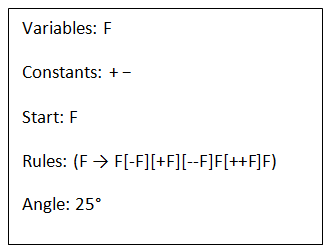
\includegraphics[width=\textwidth]{EPLCfig1a}
                \caption{L-systems algorithms.}
                \label{fig:sub1eplc1}
        \end{subfigure}
        \begin{subfigure}[b]{0.42\textwidth}
                \centering
                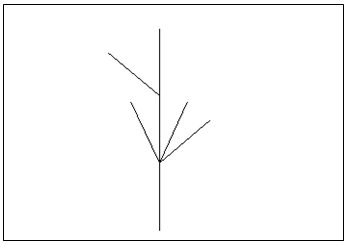
\includegraphics[width=\textwidth]{EPLCfig1b}
                \caption{The corresponding branch.}
                \label{fig:sub2eplc1}
        \end{subfigure}   
        \caption{Tree structure under L-systems.}
        \label{fig:eplc1}
\end{figure}

After giving an L-system for each branch pattern, we use an OpenGL library to draw the corresponding branch. Each fragment (see lines in Figure \ref{fig:sub2eplc1}) of a branch is described by a 3D cylinder. We then apply an angle at the joints to rotate these cylinders. Then we get a 3D branch based on L-systems algorithms. All 3D branches in the branch library have the same length and radius for every twig. When applying a branch to a tree model, we compute the length and radius by parameters from the growth point.

\subsection{Hemisphere for Probabilities Distribution}

A hemisphere controls the distribution of branches and leaves. We define it by a position, a radius, and a probability distribution. The position of this hemisphere is on the top area of a tree model. Its diameter is set by users for different purposes. For example, simulating photokinesis requires the hemisphere to be big enough to include the track of sun movement. The probability distribution divides the hemisphere into several parts and assigns probabilities of particle generation to each part. 

\begin{figure}[!t]
\centering
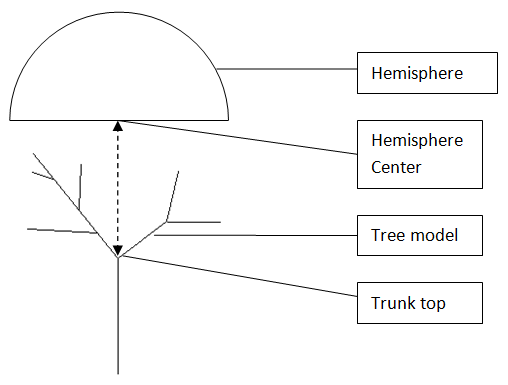
\includegraphics[scale=0.8]{EPLCfig2}
\caption{Side view of a 3D tree model and hemisphere.}
\label{fig:EPLCfig2}
\end{figure}
 
\begin{figure}[!t]
\centering
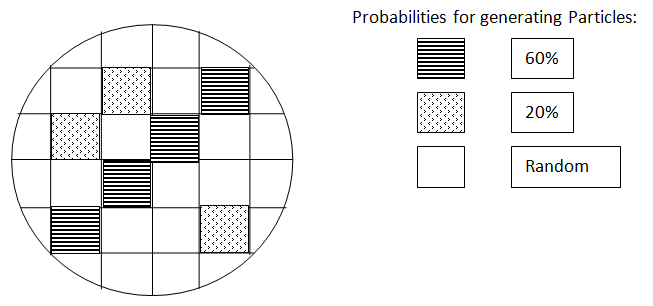
\includegraphics[scale=0.8]{EPLCfig3}
\caption[An example of probability distribution of hemisphere.]{An example of the probability distribution of a hemisphere (up view).}
\label{fig:EPLCfig3}
\end{figure} 

In Figure \ref{fig:EPLCfig2}, we show the definition of a hemisphere. The size of the hemisphere is bigger than the tree crown. The position is right next to the tree model and the center of the hemisphere is perpendicular to the top of the trunk. 

In Figure \ref{fig:EPLCfig3}, we show an example of hemisphere division and a probability distribution. We cut the hemisphere into several parts. Each part has a specific probability of generating particles. These probabilities control the shape of the 3D tree model.

The functions of the hemisphere have three parts: arranging probabilities for generating particles, defining directions for particles, and setting initial positions for particles. As in Figure \ref{fig:EPLCfig3}, these probabilities decide how particles generate in different parts. In this example, particles are mainly generated in the shaded areas. If the shaded area is the track of the sun's movement, branches in a tree mainly grow towards these areas. When generating a particle on the hemisphere, we first decide the initial position of this particle according to the probability of its region. We then give an initial direction for this particle to move in the 3D scene.

After initializing a particle and its movement in the scene, we define a landing constraint for the particle. The constraint is defined by the user. For example, we can use the nearest Cartesian distance as the constraint. The distance is from the particle's position on the hemisphere to branch top points.

After using the landing constraint to define the landing point on existing tree branches, we select a branch pattern from the L-systems branch library. Using the growth parameters of the landing point, we are able to attach the new branch to the existing tree.

\subsection{Bounding Box for Local Growth Control}

A bounding box defines the minimal 3D rectangular volume around the existing tree model. The bounding box computes the current growth space. When the tree model grows larger, the size of the bounding box grows simultaneously. Therefore, the bounding box can detect whether there are intersections between the bounding box of the tree and other objects. For example, after adding a new branch, if the tree's bounding box intersects with a rock's bounding box, we can delete this branch and generate the next branch.

The bounding box is an approximate method for defining the tree's growth area. In fact, the most exact way is to calculate all points on the tree body. However, this approach is very expensive and not necessary. In contrast, using a bounding box we only need to calculate for two points and detect the growth area approximately. Since a tree has many branches, such approximation highly reduces computations while properly detecting outer barriers.

\subsection{Growth Level Controls}

We introduce the level of growth to control the growth of branches and leaves. In Figure 4, the tree model has three growth levels. Figure 5 shows the corresponding tree model for the growth levels in Figure 4. Because natural trees grow new branches every year, the leaf sizes and colors change according to branch ages and different parts of trees. For example, the color of younger branches and leaves is light green while older ones are dark green or brown. The growth level parameter tracks the age of branches and is used to define leaf and bark appearance. When we add new branches or leaves, the age parameter indicates the right colors, sizes, and other parameters for them. 

\begin{figure}[!t]
\centering
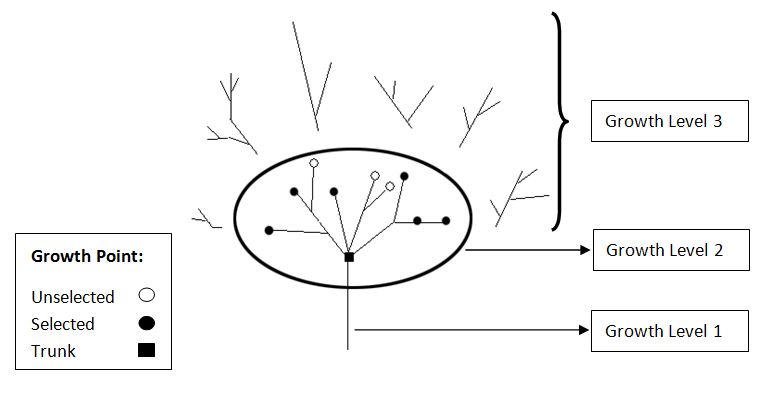
\includegraphics[scale=0.6]{EPLCfig4}
\caption[Various growth levels. ]{Growth level 1, growth level 2, and growth level 3 in a tree model.}
\label{fig:EPLCfig4}
\end{figure}

\begin{figure}[!t]
\centering
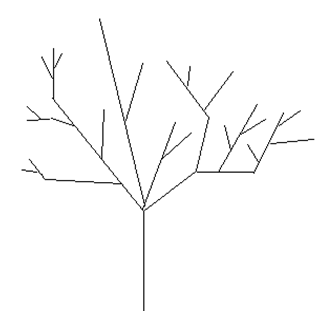
\includegraphics[scale=0.8]{EPLCfig5}
\caption{A tree model with three growth levels.}
\label{fig:EPLCfig5}
\end{figure}
 
Growth levels set different particle generations. In Figure \ref{fig:EPLCfig4}, the first generation of particles is the trunk, the oldest part in a tree, having a growth number 1. Then the second generation, branches growing on trunks, has a growth number 2. After adding growth level 3, we get a tree model as shown in Figure \ref{fig:EPLCfig5}. 

Leaves grown in these parts should have darker colors and bigger sizes than those on top, which has a higher growth number. Therefore, different growth levels can simulate different ages of branches and work as a reference for leaves.

\subsection{Tree Generation Steps}

Based on the discussed four parts---L-systems, a hemisphere, a dynamical bounding box, and growth level controls---we can generate a 3D tree model. There are three main steps in this process: (1) define the hemisphere and the branch library, (2) generate particles and control their movements, and (3) distribute the particles in a tree model. We discuss these steps below.

(1)	Define a hemisphere and a branch library.

We define the hemisphere's initial position, size, and probability distribution. The position and size is decided by the scene and the tree size while the center of the hemisphere is identical to the top of the trunk. The probability distribution is defined by users for different purposes. This distribution also reflects the projection of 3D branches on the hemisphere. Therefore, the probability distribution can control the shape of the tree.

As for the branch library based on L-systems, we define different L-systems algorithms and get different patterns of branch shapes.

(2)	Generate particles and control their movements.

We generate a certain number of particles for a growth level at the same time. For example, 10 particles for growth level 2. Then we select proper positions for these particles on the tree.

A particle denotes a branch selected from the branch library. The particle is generated on the surface of the hemisphere according to the probability distribution. With an initial position on the hemisphere and an initial orientation, the particle moves in a Brownian way in the scene.

(3) Distribute the particles in a tree model.

During the Brownian movement, the particle compares and finds a nearest distance among all growth points. Then the branch denoted by this particle is attached to this nearest growth point. After the particle settles, we calculate a new bounding box to replace the old one for this tree. However, there is one exception. After attaching the new branch to the existing tree model, if the new bounding box overlaps some outer blocks, the particle with this branch is cancelled and we then go to the next particle generation. 

After one particle is generated and distributed in a tree model, we repeat step (2) and step (3) until we reach a user-defined numbers of particles. 

\subsection{Examples of 3D Tree Modeling}

Based on this new method with L-systems, we can add more constraints to this model to simulate some properties of natural trees. Here we introduce implementations of trees' photokinesis simulations and of growth control over blocks.

\subsubsection{Trees' Photokinesis Simulations}

The photokinesis simulation relies on the probability distribution on the hemisphere. This simulation is used to make the tree branches grow towards the sun. In order to give more weight to the lighting area, we add more probability of generating tree branches in the track of sun movement. Then the hemisphere works as the sky and the probability distribution is assigned by the sun's track. Figure \ref{fig:EPLCfig6} shows one result of photokinesis simulation.
 
\begin{figure}[!t]
\centering
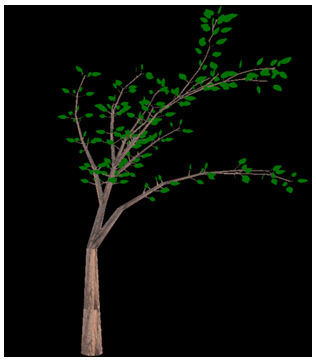
\includegraphics[scale=0.8]{EPLCfig6}
\caption{A result for photokinesis simulation.}
\label{fig:EPLCfig6}
\end{figure} 

\subsubsection{Growth Control Over Blocks}

We control the growth over blocks by using the dynamic bounding box. When simulating 3D tree growth over blocks, the tree should avoid growing in the blocked area. We use bounding boxes to control blocks, such as outer buildings or rocks. First, we calculate bounding boxes of the blocks. During steps to distribute branches, when a tree's bounding box goes into the bounding boxes of blocks, the current particle is deleted. Thus we can eliminate tree branches grown in the blocked areas.

\subsubsection{Trees' Fruits Simulation}

We can add fruits on a tree using this method. The process of fruits simulation is similar to the leaf attachment. We define the size, shape, and color for fruits. Then we generate particles on the probability hemisphere and distribute the fruits to different growth levels according to the tree model.

\section{Results} 

This new method works well and has some advantages. This model controls the local shape of branches using L-systems and the global shape of trees using the probability hemisphere. Different growth levels approximately simulate the growth process. The bounding box detects outer obstacles. We analyze these characters in detail below. 

\subsection{Growth Probability Control by Hemisphere}

This method introduces a hemisphere control over tree growth by distributing particle probabilities. The tree shape is decided by the predefined probabilities on the surface of this hemisphere. As we use a particle system to control the distributions of branches, the particles' initial sizes and orientations are defined on this hemisphere. Thus, the main shape of a tree is decided and we can use different types of branch patterns to generate the details.
Figure \ref{fig:EPLCfig7} shows two types of hemisphere control on tree shape. In Figure \ref{fig:EPLCfig7}(a), all branches are grown towards the same direction. In Figure \ref{fig:EPLCfig7}(b), there is only one priority growth direction.

\begin{figure}[!t]
\centering
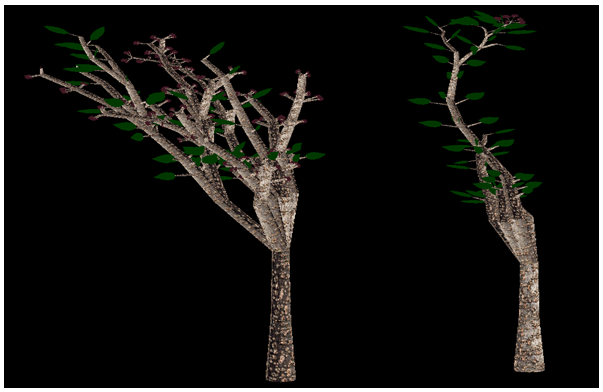
\includegraphics[scale=0.8]{EPLCfig7}
\caption[Branch directions. ]{(a) Branches towards the same direction; (b) branches clustered together for one direction.}
\label{fig:EPLCfig7}
\end{figure}

\subsection{Growth Level Controls}

We introduce a new conception of growth level controls. In this control, we give different growth levels for different branches, leaves, and even fruits with different ages. Branches, leaves, and fruits with the same growth level can share some parameters, such as sizes, colors, and shapes.
In Figure \ref{fig:EPLCfig8}, we show two results for the growth level work. In Figure \ref{fig:EPLCfig8}(a), this tree model has needle-shaped leaves and heart-shaped leaves. It also has small red flowers on the top level. In Figure \ref{fig:EPLCfig8}(b), we add some fruits to this tree model.

\begin{figure}[!t]
\centering
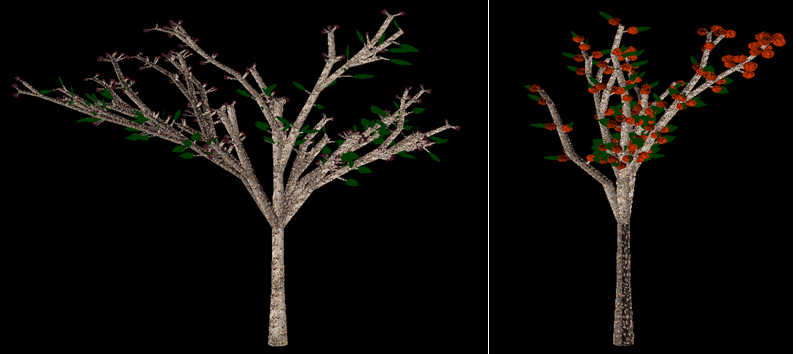
\includegraphics[scale=0.6]{EPLCfig8}
\caption[3D tree models.]{(a) A 3D tree model with different leaf shapes and flowers; (b) A 3D tree model with fruits.}
\label{fig:EPLCfig8}
\end{figure}

\subsection{Growth Control over Small Components}

This new method has advantages in controlling small components in a tree. Compared to the DLA (Diffusion-Limited Aggregation) method \cite{Vicsek1992,Kim2007} for tree modeling, our method reduces computing work by reducing the particles. Using a branch type as a particle rather than assigning a DLA particle for every twig, fewer particles are needed for the same number of twigs in a tree. Since computation for each DLA particle is the same, fewer DLA particles requires less computation. In Figure \ref{fig:EPLCfig9}, we have the same tree shape. If we use traditional DLA in Figure \ref{fig:sub1EPLCfig9}, the circled branch needs three particles to calculate. But in Figure \ref{fig:sub2EPLCfig9}, we calculate one DLA particle for three twigs in one branch unit.
 
\begin{figure}
\centering
        \begin{subfigure}[b]{0.7\textwidth}
                \centering
                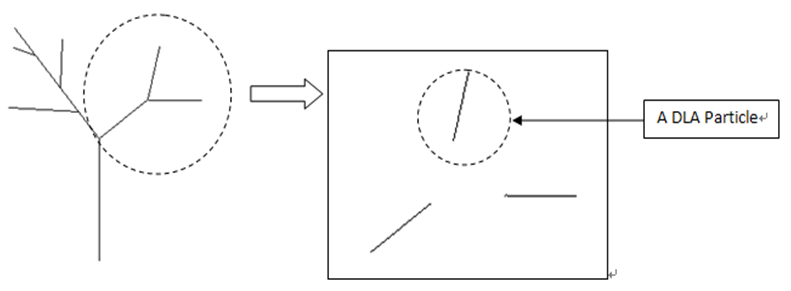
\includegraphics[width=\textwidth]{EPLCfig9a}
                \caption{DLA particles.}
                \label{fig:sub1EPLCfig9}
        \end{subfigure}
        \begin{subfigure}[b]{0.7\textwidth}
                \centering
                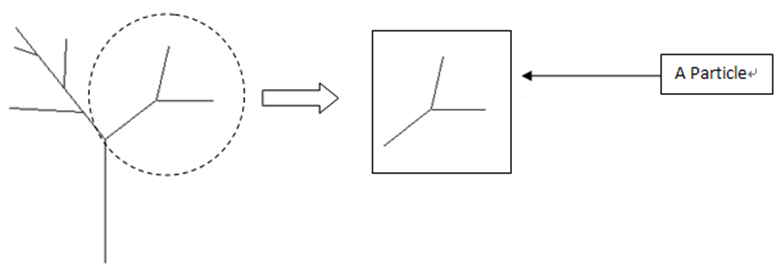
\includegraphics[width=\textwidth]{EPLCfig9b}
                \caption{Particles in our method.}
                \label{fig:sub2EPLCfig9}
        \end{subfigure}   
        \caption{Particles with tree shape.}
        \label{fig:EPLCfig9}
\end{figure} 

\subsection{Growth Control for Leaves}

Our method provides a new method of leaf simulation, which is difficult for most current methods. Leaf simulation is difficult to achieve by L-systems because L-systems can't control the positions of leaves randomly on branches. Even the popular image-based approaches have difficulties handling leaf simulation. These approaches usually generate branches very well. However, after branch construction, leaves are added randomly and often can't attach to the branches. Our method uses the hemisphere to handle the overall distribution of leaves in a tree, and we apply growth level controls to define leaves with different shapes, sizes, and colors according to the branch properties to which they attach.

This approach is also effective. We only need to change leaf parameters according to the numbers of total growth levels. At a certain growth level, we define the shapes, sizes, and colors for leaves in that level. As for the whole tree, branches have leaves of the same age. In the natural world, that means the old branches have old and big leaves while young branches have young and small leaves in the same shapes.

\subsection{Growth Control by Bounding Box}

Using dynamic bounding boxes in detecting proper positions for DLA particles gives flexible controls over 3D tree models. We generate the DLA particle in the bounding box and find a position in this bounding box. By controlling this bounding box, we can control the growth of the tree. For example, if the current bounding box overlaps a building's bounding box, the current DLA particle should be canceled.

Figure \ref{fig:EPLCfig10} shows an example of tree growth. In this example, the 3D tree model tries to avoid the white box to grow. This process is similar to the process of a tree growing to avoid outer barriers such as bridges or buildings.

\begin{figure}[!t]
\centering
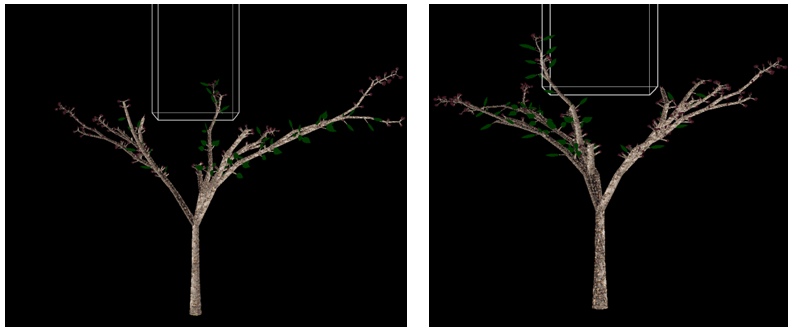
\includegraphics[scale=0.6]{EPLCfig10}
\caption[Simulate tree growth. ]{Trees grow to avoid the white outer box viewed from two different directions.}
\label{fig:EPLCfig10}
\end{figure} 

\subsection{Randomness}

Compared to traditional L-systems, our method generates tree models with more random shapes. Every branch unit carries an L-system algorithm. Because particles control every branch unit, the whole tree doesn't follow any L-systems algorithms. This approach solves artificial iterations from single pure L-system algorithms. In Figure \ref{fig:EPLCfig11}, (a) is a tree model from the combination method and (b) is from a traditional L-systems algorithm. Figure \ref{fig:EPLCfig11}(a) has a random look while (b) has a self-similar character that makes the tree model artificial.

\begin{figure}[!t]
\centering
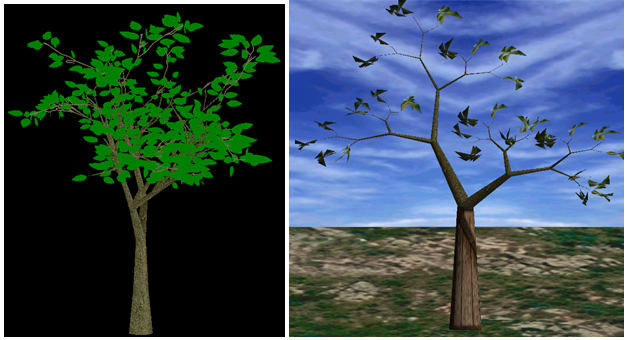
\includegraphics[scale=0.8]{EPLCfig11}
\caption[3D tree model compared to L-system. ]{(a) Combination method tree; (b) traditional L-systems tree.}
\label{fig:EPLCfig11}
\end{figure} 

Randomness from the DLA method goes too far for tree modeling. As shown in Figure \ref{fig:EPLCfig12}, the shape from (b) might be more curved than is common in trees. Using the combination method, we can reduce the curvature by reducing the number of particles, which stand for L-systems branch units rather than twigs. 

\begin{figure}[!t]
\centering
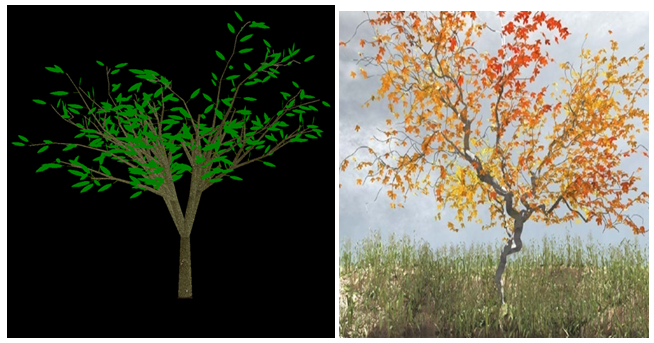
\includegraphics[scale=0.8]{EPLCfig12}
\caption[3D tree model compared to DLA. ]{(a) Combination method tree; (b) traditional DLA tree.}
\label{fig:EPLCfig12}
\end{figure} 

\section{Conclusions and Discussions} 

We introduce a new method based on L-systems for 3D tree models. In this method, a hemisphere controls probability distributions for branches, leaves, and fruits; growth level controls the distributions for different ages of branches; and a bounding box detects the outer collisions. This new method employs a moving particle for a branch unit, which reduces computation costs of traditional methods like DLA. The hemisphere controls the probability distributions to simulate some natural properties of trees or some special effects. The growth level can manage the internal growth in a tree through age controls. In the tree construction process, the bounding provides an easy and efficient way to control tree growth. Therefore, we can manage the main shapes using the hemisphere while controlling the internal growth through growth level controls. Under these controls, randomness is added by randomly selected tree branches from the L-systems branch library.

The future work in this research may focus on adding more controls over particle movements. We can try to find some more efficient approaches for distributing L-systems branch units. We can also simulate tree animations using this model. Furthermore, we can apply forestry equations to make tree models follow real growth rules.

\section{Practical Application Plan} 

In this paper, we present an innovative method on 3D tree modeling. Tree modeling is a hot research topic in both forestry and computer graphics. This new method with L-systems can produce a user-defined or random 3D tree model. With this tree modeling method, we can control every part in a 3D tree model, including trunks, branches, leaves, flowers, and fruits. For these parts, we can change colors, textures, and shapes very flexibly. The second advantage is about the level control. Based on this control, parts in a tree with different ages look different. The third advantage is the possibility of hemi-sphere control. This is a new method for controlling the shape of a tree by controlling the probable distribution of particles on this hemisphere. Because of the advantages of this new method, it might have three effects: social, political, and economic, which are discussed below.

However, since this new method is currently a basic idea, further work focused on different application areas is need to achieve these goals.

\subsection{Social Effects}

There are two main aspects of this new 3D tree modeling method that have social effects. One is the innovation of this method. Another is the use of this 3D tree model in our society.  

The innovation of this method provides a new method for 3D tree generating. It can help researchers to understand tree modeling and even find better solutions. This new method takes advantage of traditional L-systems and solves the problems with L-systems. We also introduce a new approach using hemisphere and level control. What's more, the bounding box technique can also be applied to this 3D tree model for detecting outer collisions of growth.

This new method can also be used in less technical communities. Based on our idea, we can produce more types of trees and control all parts in a tree. If this method can be applied to work as a demo in some community or school, it helps more people to know how trees grow in a computer. Furthermore, if more biological characters are added, forestry researchers can use this model to predicate the growth of trees and then evaluate the wood productions. However, in addition to our tree model, more work is needed to do to achieve these social effects. 

\subsection{Political Effects}

This model has little effect on politics. However, we suggest this tool for governing trees in a forestry department. At present, most forestry departments use a database or even paper to record and manage trees. With our 3D tree model, we can display these data in visual 3D and thus get more direct information from these data. Therefore, our new method, if there are any political effects, can help forestry departments and researchers to get more information from tree data and help to make some decisions. 

\subsection{Economic Effects}

One reason for the interest in 3D trees is the wide applicability and economic value. As a product of this simulating tool, the automatic generated tree model can reduce manual work and achieve a good simulating result. Our 3D tree model can be used in commercial 3D games, commercial software of tree models, city planning, and so on. 

In commercial 3D games, our tree model can set up a good scene or background. If further work can be done, we will try to improve the efficiency of the current model to make it more applicable.

In commercial software, the method for generating a 3D tree shape is important. Current 3D tree modeling software, such as XFrog, has a great market. Our method suggests a new method of 3D tree modeling and is easy to control. Since this model can also be used in 3D tree modeling software, the method has potential economic value in software design.

In city planning, we can use different shapes of 3D tree models to view corresponding designs. For example, when we choose a type of tree for use on a street, we can generate different 3D tree shapes to make comparisons.